\section{Heap Sort}

\subsection{Alberi}
\begin{itemize}
    \item binario: ogni nodo ha al massimo due figli.
    \item altezza: distanza dalla radice alla foglia più distante.
    \item ordinato: ogni nodo ha un figlio minore o uguale a se stesso.
\end{itemize}

\subsection{Alberi completi}
\begin{mdframed}
    \textbf{Albero binario completo:} ogni nodo non foglia ha due figli e ogni cammino radice-foglia ha la stessa lunghezza.
\end{mdframed}
\begin{equation*}
    \text{\# nodi} = \sum_{i=0}^k 2^i -1 \quad (h = \text{altezza})
\end{equation*}
\begin{center}
    \begin{tabular}{c}
        \\ 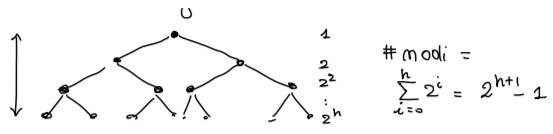
\includegraphics[width=0.6\textwidth]{image/AlberoCompleto.png} \\ \\
    \end{tabular}
\end{center}

\subsection{Alberi quasi completi}
\begin{mdframed}
    \textbf{Albero quasi completo:} ogni livello è completo, tranne eventualmente l’ultimo con foglie tutte a sx.
\end{mdframed}
\begin{center}
    \begin{tabular}{c}
        \\ 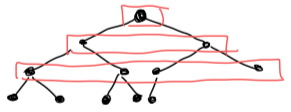
\includegraphics[width=0.3\textwidth]{image/AlberoQuasiCompleto.png} \\ \\
    \end{tabular}
\end{center}

\subsection{Heap}
\begin{mdframed}
    \textbf{Heap:} albero binario ordinato quasi completo, ma implementato come se fosse un array.
\end{mdframed}
\paragraph{Caratteristiche:}
\begin{itemize}
    \item $A[1]$ è radice
    \item Un generico nodo sta in posizione $A[i]$.
    \item Un nodo $A[2i]$ è il figlio sinistro del nodo $A[i]$
    \item Un nodo definito come nodo parent/genitore sta in posizione $A[i/2]$
    \item Lo spazio occupato effettivamente è $A.size$, la lunghezza dell'array è $A.length$.
\end{itemize}

\begin{center}
    \begin{tabular}{c}
        \\ 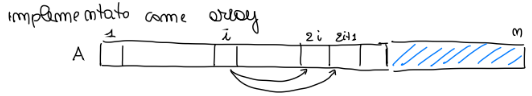
\includegraphics[width=0.6\textwidth]{image/Heap.png} \\ \\
    \end{tabular}
\end{center}

\paragraph{Max Heap}
Il Max Heap è un Heap dove:
\begin{itemize}
    \item $\forall A[i], A[i] \geq$ nodi discendenti (quindi, $A.Left[i]$,$A.Right[i]$)
    \item $\forall A[i], A[i] \leq$ nodi antenati (quindi, $A[i] \leq A.Parent[i]$)
\end{itemize}

\begin{center}
    \begin{tabular}{c}
        \\ 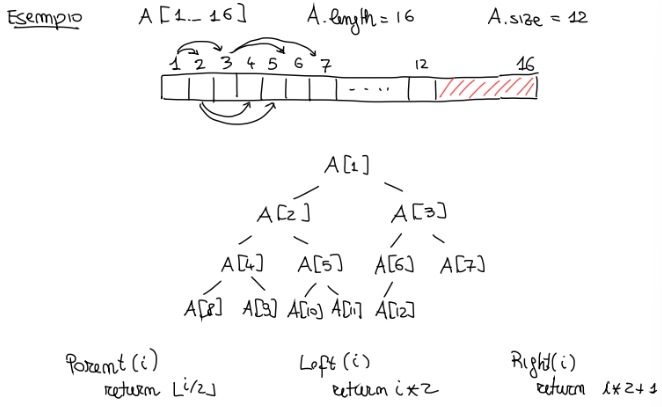
\includegraphics[width=0.7\textwidth]{image/HeapSortExample.png} \\ \\
    \end{tabular}
\end{center}

\subsection{Pseudocodice}
\begin{mdframed}
\begin{lstlisting}[language=C]
MAX-HEAPIFY(A)
1   l = LEFT(i)
2   r = RIGHT(i)
3   if l<=A.heapsize and A[l] > A[i]
4       max = l
5   else
6       max = i
7   if r<=A.heapsize and A[r] > A[max]
8       max = r
9   if max != i
10      A[i] <-> A[max]
11      MAX-HEAPIFY(A,max)
\end{lstlisting}
\end{mdframed}

\subsection{Complessità}
Dipende dall'albero, il quale avrà $n$ elementi possibili:
\begin{itemize}
    \item la complessità $O(h)$, con $h$ altezza del sottoalbero, alternativamente $O(\log(n))$.
    \begin{equation*}
        \begin{rcases}
            n \geq 2^{2^{h-1}+1} + 1 = 2^h \\
            h \leq \log_2n \\
        \end{rcases}
        \Rightarrow O(h) \;\tilde{=}\; O(\log n)
    \end{equation*}
    \item se invece fosse visto come ricorrenza, si può dimostrare con il Master Theorem
\end{itemize}




\newpage